\documentclass[10pt,twocolumn]{article}
\usepackage[margin=0.75in]{geometry}
\usepackage[T1]{fontenc}
\usepackage{lmodern,amsmath,amssymb,graphicx,booktabs,url}
\usepackage[hidelinks]{hyperref}
\title{Coverage vs.\ Mutation Feedback for Improving Student JUnit Tests:\\ A Crossover Study on Held-Out Wrong Answer Submissions}
\author{Pham Nhat Thang \and Tran Trieu Tien \and Ngo Minh Tien \and Phung Thanh Nhan\\
\small FPT University, Ho Chi Minh City, Vietnam}
\date{}
% Bảng và hình trải hết hai cột
\let\origtable\table \let\endorigtable\endtable
\renewenvironment{table}[1][t]{\begin{table*}[#1]}{\end{table*}}
\renewenvironment{figure}[1][t]{\begin{figure*}[#1]}{\end{figure*}}
\begin{document}
\twocolumn[\maketitle\vspace{-2em}]
\begin{abstract}
This study compares feedback from a coverage tool (JaCoCo) and a mutation testing tool (PITest) on how well each helps students write tests that catch real faults. In a crossover experiment, 24 participants each had 20 minutes to add JUnit tests to two IBM CodeNet programs, using one tool per program. The outcome measure was the gain in detection rate on held-out Wrong Answer submissions. The two tools did not differ (Hodges--Lehmann estimate $-$0.012, 95\% CI [$-$0.118, 0.074], Wilcoxon p = 0.483, N = 22). Two problems showed up in the data. Most newly written tests were invalid, mainly because of wrong expected values. With its default configuration, PITest stopped without producing a report in 58 of 96 runs, because the test suite contained tests that failed on the program under test. These preliminary results suggest educators should teach students to write valid tests and adjust the PITest configuration, instead of choosing between report types. The study is exploratory and needs confirmation with real students and the planned sample of 48.
\end{abstract}

\IfFileExists{sections/01_introduction.tex}{\section{Introduction}
\label{sec:intro}

The study had 24 participants.

In software testing courses, students often write a JUnit test suite for a program and then add tests based on feedback from a tool. The two most common kinds of feedback are branch coverage and mutation testing. JaCoCo shows which branches in the source code no test has executed. PITest creates small faulty versions of the program (mutants) and lists the mutants the test suite has not detected. Both suggest which tests to write next. The purpose of writing tests is to catch faults; coverage and mutation score measure this only indirectly.

Studies on open-source projects found that, once test suite size is controlled for, coverage has only a low to moderate correlation with fault detection~\cite{inozemtseva2014}, and mutation score is also only weakly correlated with detecting real faults~\cite{papadakis2018}. In education, existing comparisons of the two kinds of feedback all use between-group or between-semester designs, small samples, and test suite quality as the outcome~\cite{mansur2024,alonge2025}. Practice time is limited, so instructors need to know which kind of feedback helps students write tests that catch more real faults.

This study compares the two kinds of feedback within the same person, under the same time budget, using real held-out Wrong Answer (WA) submissions as the outcome. The research question is:

\textbf{RQ1.} Within the same time budget for adding tests, how do uncovered-branch feedback from JaCoCo (condition J) and surviving-mutant feedback from PITest (condition P) differ in the gain in detection rate of held-out Wrong Answer submissions, relative to the participant's own initial JUnit suite?

The study makes three contributions: (1) a non-self-confirming measure, $\Delta\mathrm{WADR}$, based on real WA submissions that participants never see, used instead of the coverage or mutation score that the two tools themselves report; (2) results of an exploratory crossover experiment with 24 participants on 12 Java problems from IBM CodeNet, reported with effect sizes and confidence intervals even though $H_0$ was not rejected; (3) public problem selection criteria, frozen data, grading scripts and analysis for reproduction.

The rest of the paper is organised as follows. Section~\ref{sec:related} presents related work, Section~\ref{sec:methods} describes the method, Section~\ref{sec:results} reports the results, Section~\ref{sec:discussion} discusses them, Section~\ref{sec:threats} covers threats to validity and Section~\ref{sec:conclusion} concludes.
}{}
\IfFileExists{sections/02_related_work.tex}{\section{Related Work}
\label{sec:related}

\subsection{Measuring the quality of student test suites}
Many studies use coverage, mutants or faulty student submissions to grade test suites. Aaltonen et al.~\cite{aaltonen2010} found that most students reached the maximum coverage score while mutation scores were more spread out. Edwards and Shams~\cite{edwards2014} and Shams~\cite{shams2015} compared test quality measures using real faults in student programs as the reference and found that coverage is not strongly correlated with fault detection. Perretta et al.~\cite{perretta2022}, on 2,711 submissions, found that mutation score correlates strongly with detecting hand-seeded faults and fairly strongly with detecting faulty student submissions. Hall and Baniassad~\cite{hall2022} found that students graded by mutation analysis wrote more correct tests. These studies evaluate how test suites are graded. They do not compare the kind of feedback students see while writing tests.

\subsection{Feedback type as an intervention}
Mansur et al.~\cite{mansur2024} compared semesters that used only coverage with one semester that used mutation testing and found better test suites and code in the latter. Mansur et al.~\cite{mansur2026} went on to compare three semesters and reported that the original PIT report did not meet students' needs without modification and additional training. Alonge~\cite{alonge2025} randomly assigned 10 students to branch or mutation feedback and measured them with tests taken before and after, without feedback; the mutation group increased its rate of catching conceptual mutants by about 0.11 and the branch group by about 0.06. Shin and Kazerouni~\cite{shin2024} interviewed 12 students using think-aloud and found that mutation feedback easily causes cognitive overload. Cordova et al.~\cite{cordova2021} and Potter et al.~\cite{potter2025} showed that how feedback is presented (conceptual level, scaffolding, visualisation) affects outcomes. Overall, the evidence leans towards mutation feedback, but it comes from small samples, between-group or between-semester designs, and test suite quality as the outcome.

\subsection{Coverage, mutants and real faults}
Inozemtseva and Holmes~\cite{inozemtseva2014} found only a low to moderate correlation between coverage and test suite effectiveness when the number of tests is controlled for. Just et al.~\cite{just2014} found that detecting mutants is significantly correlated with detecting real faults, independently of coverage. Papadakis et al.~\cite{papadakis2018} found this correlation to be weak when test suite size is controlled for. For this reason, this study uses real faults as the outcome and includes test suite size in the analysis.

\subsection{Differences from the closest work}
Compared with Alonge~\cite{alonge2025}, this study asks a different question: how effectively tests are added while feedback is available, rather than skill transfer. It uses a within-person crossover design instead of two groups, uses Java and JUnit, and measures with real WA submissions instead of designer-made mutants. Shin and Kazerouni~\cite{shin2024} also had the same person use several kinds of feedback, but theirs is a qualitative study and does not measure detection of faulty submissions.
}{}
\IfFileExists{sections/03_methodology.tex}{\section{Method}
\label{sec:methods}

The study had 24 participants at three experience levels (4 fresher, 15 junior, 5 semi-senior), assigned to the schedule at random with seed 2026.

\subsection{Design}
The study used a crossover design. Each participant completed two sessions on two different problems, one with JaCoCo (J) and one with PITest (P). The schedule balanced tool order: half did J first and half did P first, and each combination of problem, session and tool appeared exactly once. No one worked on the same problem with both tools. The planned sample was 48, with a minimum of 24. Because there were only 24 participants, the study is reported as exploratory.

\subsection{Data}
Problems were taken from IBM CodeNet~\cite{puri2021}. A problem was eligible if it had Sample Input/Output, a unique correct answer, at least 30 Java Accepted and 30 Java Wrong Answer submissions, and a median Accepted code size of at most 2,000 bytes (722 of 4,053 problems qualified). Problems were drawn in random order (seed 2026) until 12 were selected, skipping problems where the Sample tests already detected every WA submission. Each problem has one program under test (PUT), an Accepted submission chosen by public criteria so that both reports still contain at least one item that the reference inputs can cover or kill. In total, 1,639 WA submissions were used for evaluation. The WA list, the reference inputs and four reference Accepted solutions per problem were locked with SHA-256 before the runs.

\subsection{Session procedure}
Participants read the problem statement and the program, then wrote an initial JUnit suite (Before) in 15 minutes without feedback. They then ran the tool of their assigned condition, read the report and added tests. Each session had four tool runs; the extended suite (After) was saved at 15, 20 and 30 minutes. The main analysis uses $T = 20$ minutes, the value kept after the mini-pilot, and tool running time counts towards $T$. JaCoCo 0.8.12 and PITest 1.16.1 ran with their default configurations, and no report items were filtered.

\subsection{Grading}
The grader compiles the test suite, runs it twice on the PUT and runs each test on its own. A test is valid if it passes both times, passes when run alone and uses only inputs within the problem constraints. Valid tests are also run on the four reference Accepted solutions; a test that fails on at least one of them is a disagreeing test. A WA submission is detected when at least one valid test fails on an assertion in both runs. The grader was verified beforehand on a constructed problem with known outcomes (80 of 80 checks matched).

\subsection{Measures}
WADR is the proportion of WA submissions in the locked list that the test suite detects. $\Delta\mathrm{WADR} = \mathrm{WADR(After)} - \mathrm{WADR(Before)}$. For each participant, $d = \Delta\mathrm{WADR}(P) - \Delta\mathrm{WADR}(J)$; $d > 0$ favours PITest. Coverage and mutation score are not the primary measure because they are the information the two tools give participants.

\subsection{Analysis}
$H_0$: $\theta = 0$ and $H_1$: $\theta \neq 0$, where $\theta$ is the pseudo-median of $d$. The main test is the two-sided paired Wilcoxon signed-rank test, with zero differences handled by Pratt's method~\cite{pratt1959}. $\theta$ is estimated with the Hodges--Lehmann estimator~\cite{hodges1963} with a 95\% confidence interval; the effect size is the rank-biserial $r$. The practical significance threshold $\delta = 0.10$ was fixed in advance. A difference is concluded when $p < 0.05$ and $|\hat{\theta}| \geq \delta$. Sessions whose Before suite did not compile were kept with $\mathrm{WADR(Before)} = 0$; sessions whose After suite did not compile were excluded from the main analysis and counted as $\mathrm{WADR(After)} = 0$ in a sensitivity analysis. Supplementary analyses covered $T = 15$ and 30 minutes, a mixed model with condition, session order and problem as fixed effects and participant as a random effect, a $2\times2$ crossover regression, $\delta = 0.05$ and 0.15, and subgroups by initial WADR. These rules were recorded before the results were seen.
}{}
\section{Results}
\label{sec:results}

\subsection{Participants and valid data}
All 24 participants completed both sessions, so all 48 scheduled sessions took place, and every one matched the frozen schedule and the SHA-256-locked WA manifests (\texttt{full\_analysis.ipynb}, Section 1).
The planned sample was 48 participants with a minimum of 24, so, following the protocol, this study is reported as exploratory.
Two participants were excluded from the paired analysis because their PITest session ended with an After suite that did not compile at T = 20 minutes (failure type \textit{method}); their JaCoCo sessions were excluded with them.
This leaves N = 22 of 24 participants (91.7\%) in the main analysis (Table~\ref{tab:excluded}).
Two PITest sessions started from a Before suite that did not compile (one of them is SV14-1 above); following the protocol, such sessions are kept with WADR(Before) = 0.

\subsection{RQ1: J versus P}
\textbf{RQ1.} Within the same time budget, how do uncovered-branch feedback from JaCoCo (condition J) and surviving-mutant feedback from PITest (condition P) differ in the gain in detection rate of held-out Wrong Answer submissions, relative to the participant's own initial JUnit suite?
$H_0$: $\theta$ = 0; $H_1$: $\theta$ $\neq$ 0, where $\theta$ is the pseudo-median of d = $\Delta$WADR(P) - $\Delta$WADR(J).

\textit{Descriptive statistics.}
In condition J, $\Delta$WADR had a median of 0.044 (IQR 0.000 to 0.198, range 0.000 to 0.750, 24 sessions); in condition P, the median was 0.000 (IQR 0.000 to 0.225, range $-$0.130 to 0.667, 22 sessions) (Table~\ref{tab:main}, Fig.~\ref{fig:dist}).
$\Delta$WADR was zero in 9 of 24 J sessions and 11 of 22 P sessions, and negative in one P session.
Across the 22 participants, the paired difference d had a median of $-$0.005 (IQR $-$0.174 to 0.061); 7 participants had $d > 0$, 11 had $d < 0$ and 4 had $d = 0$.
The distribution of d showed no strong asymmetry (skewness 0.26; Fig.~\ref{fig:dist}, right).

\textit{Test and effect size.}
The two-sided Wilcoxon signed-rank test (Pratt treatment of zeros, normal approximation because of zero differences) gave W = 100, p = 0.483.
The Hodges--Lehmann estimate was $\hat{\theta}$ = $-$0.012 with a 95\% confidence interval of [$-$0.118, 0.074], and the matched-pairs rank-biserial correlation was r = $-$0.16 (small).
Since p $\geq$ 0.05 and $|\hat{\theta}| < \delta$ = 0.10, we fail to reject $H_0$: no difference between J and P was found for RQ1.
The interval includes differences as large as 0.12 in favour of JaCoCo and 0.07 in favour of PITest.

\subsection{Pre-specified supplementary and sensitivity analyses}
All analyses specified in the protocol led to the same conclusion as the main analysis (Table~\ref{tab:sens}).
Counting an After suite that does not compile as WADR = 0 (N = 24) gave $\hat{\theta}$ = $-$0.016, p = 0.350.
Using T = 15 or T = 30 minutes gave $\hat{\theta}$ between $-$0.016 and 0.000 with p $\geq$ 0.350.
A linear mixed model with condition, session order and problem as fixed effects and participant as a random effect estimated the effect of P at $-$0.010 (95\% CI [$-$0.101, 0.081], p = 0.829; 46 sessions); adding the number of independent inputs or WADR(Before) as covariates gave $-$0.028 and $-$0.010.
In the 2$\times$2 crossover regression, the order-adjusted effect was $-$0.021 ([$-$0.130, 0.089]) and the period effect was 0.004 (p = 0.934).
The conclusion did not change when we kept all tests that disagreed with the reference Accepted solutions, when we counted WA submissions detected through an exception (secondary measure), or when we dropped participants whose problem had more items that the reference inputs could not cover or kill than items they could (N = 10).
The conclusion was also the same with $\delta$ = 0.05 and $\delta$ = 0.15.
In the subgroups below and above the median initial WADR (11 participants each), $\hat{\theta}$ was $-$0.016 and $-$0.001 (both p $\geq$ 0.27).
Per-problem means of $\Delta$WADR are shown in Fig.~\ref{fig:problem}; each problem had one or two sessions per condition, so no per-problem tests were run.

\textit{Feedback received.} JaCoCo produced a report in all 96 tool runs (24 sessions $\times$ 4 runs).
PITest produced a report in 30 of 96 runs (12 of 24 first runs); in 58 runs it stopped because at least one test failed on the program under test, and in 8 runs the suite did not compile.
In an exploratory analysis restricted to the 11 participants whose PITest session received at least one report, $\hat{\theta}$ = $-$0.020 ([$-$0.212, 0.180], p = 0.623).
No session reached the ceiling in condition J (WADR(After) $\geq$ 0.95 in 0 of 24), and one did in condition P (1 of 22).
Three tests in one JaCoCo session disagreed with the reference Accepted solutions; WADR was the same whether they were kept or removed.

\begin{table}[t]
\centering
\caption{RQ1: $\Delta$WADR at $T = 20$ minutes by condition and the paired comparison ($N = 22$ participants).}
\label{tab:main}
\begin{tabular}{lccccc}
\hline
 & Sessions & Median (IQR) & $p$ & $\hat{\theta}$ [95\% CI] & $r$ \\
\hline
J (JaCoCo) & 24 & 0.044 (0.000--0.198) & & & \\
P (PITest) & 22 & 0.000 (0.000--0.225) & & & \\
$d = P - J$ & 22 pairs & $-0.005$ ($-0.174$--$0.061$) & \textbf{0.483} & \textbf{$-0.012$ [$-0.118$, $0.074$]} & $-0.16$ \\
\hline
\end{tabular}
\end{table}

\begin{table}[t]
\centering
\caption{Sensitivity and supplementary analyses for RQ1. Rows marked $^{\dagger}$ are exploratory.}
\label{tab:sens}
\begin{tabular}{lccc}
\hline
Analysis & $N$ & $\hat{\theta}$ [95\% CI] & $p$ \\
\hline
Main ($T = 20$, non-compiling After excluded) & 22 & $-0.012$ [$-0.118$, $0.074$] & 0.483 \\
Non-compiling After counted as 0 & 24 & $-0.016$ [$-0.126$, $0.063$] & 0.350 \\
$T = 15$ & 23 & $0.000$ [$-0.090$, $0.141$] & 0.927 \\
$T = 30$ & 22 & $-0.012$ [$-0.129$, $0.074$] & 0.504 \\
Keep tests disagreeing with Accepted solutions & 22 & $-0.012$ [$-0.118$, $0.074$] & 0.483 \\
Secondary measure (exception counts as detection) & 22 & $-0.019$ [$-0.130$, $0.074$] & 0.407 \\
Drop problems with many unreachable report items & 10 & $-0.005$ [$-0.189$, $0.083$] & 0.716 \\
Mixed model, coefficient of P (sessions) & 46 & $-0.010$ [$-0.101$, $0.081$] & 0.829 \\
Crossover regression, order-adjusted & 22 & $-0.021$ [$-0.130$, $0.089$] & 0.700 \\
Participants with $\geq 1$ PITest report$^{\dagger}$ & 11 & $-0.020$ [$-0.212$, $0.180$] & 0.623 \\
\hline
\end{tabular}
\end{table}

\begin{figure}[t]
\centering
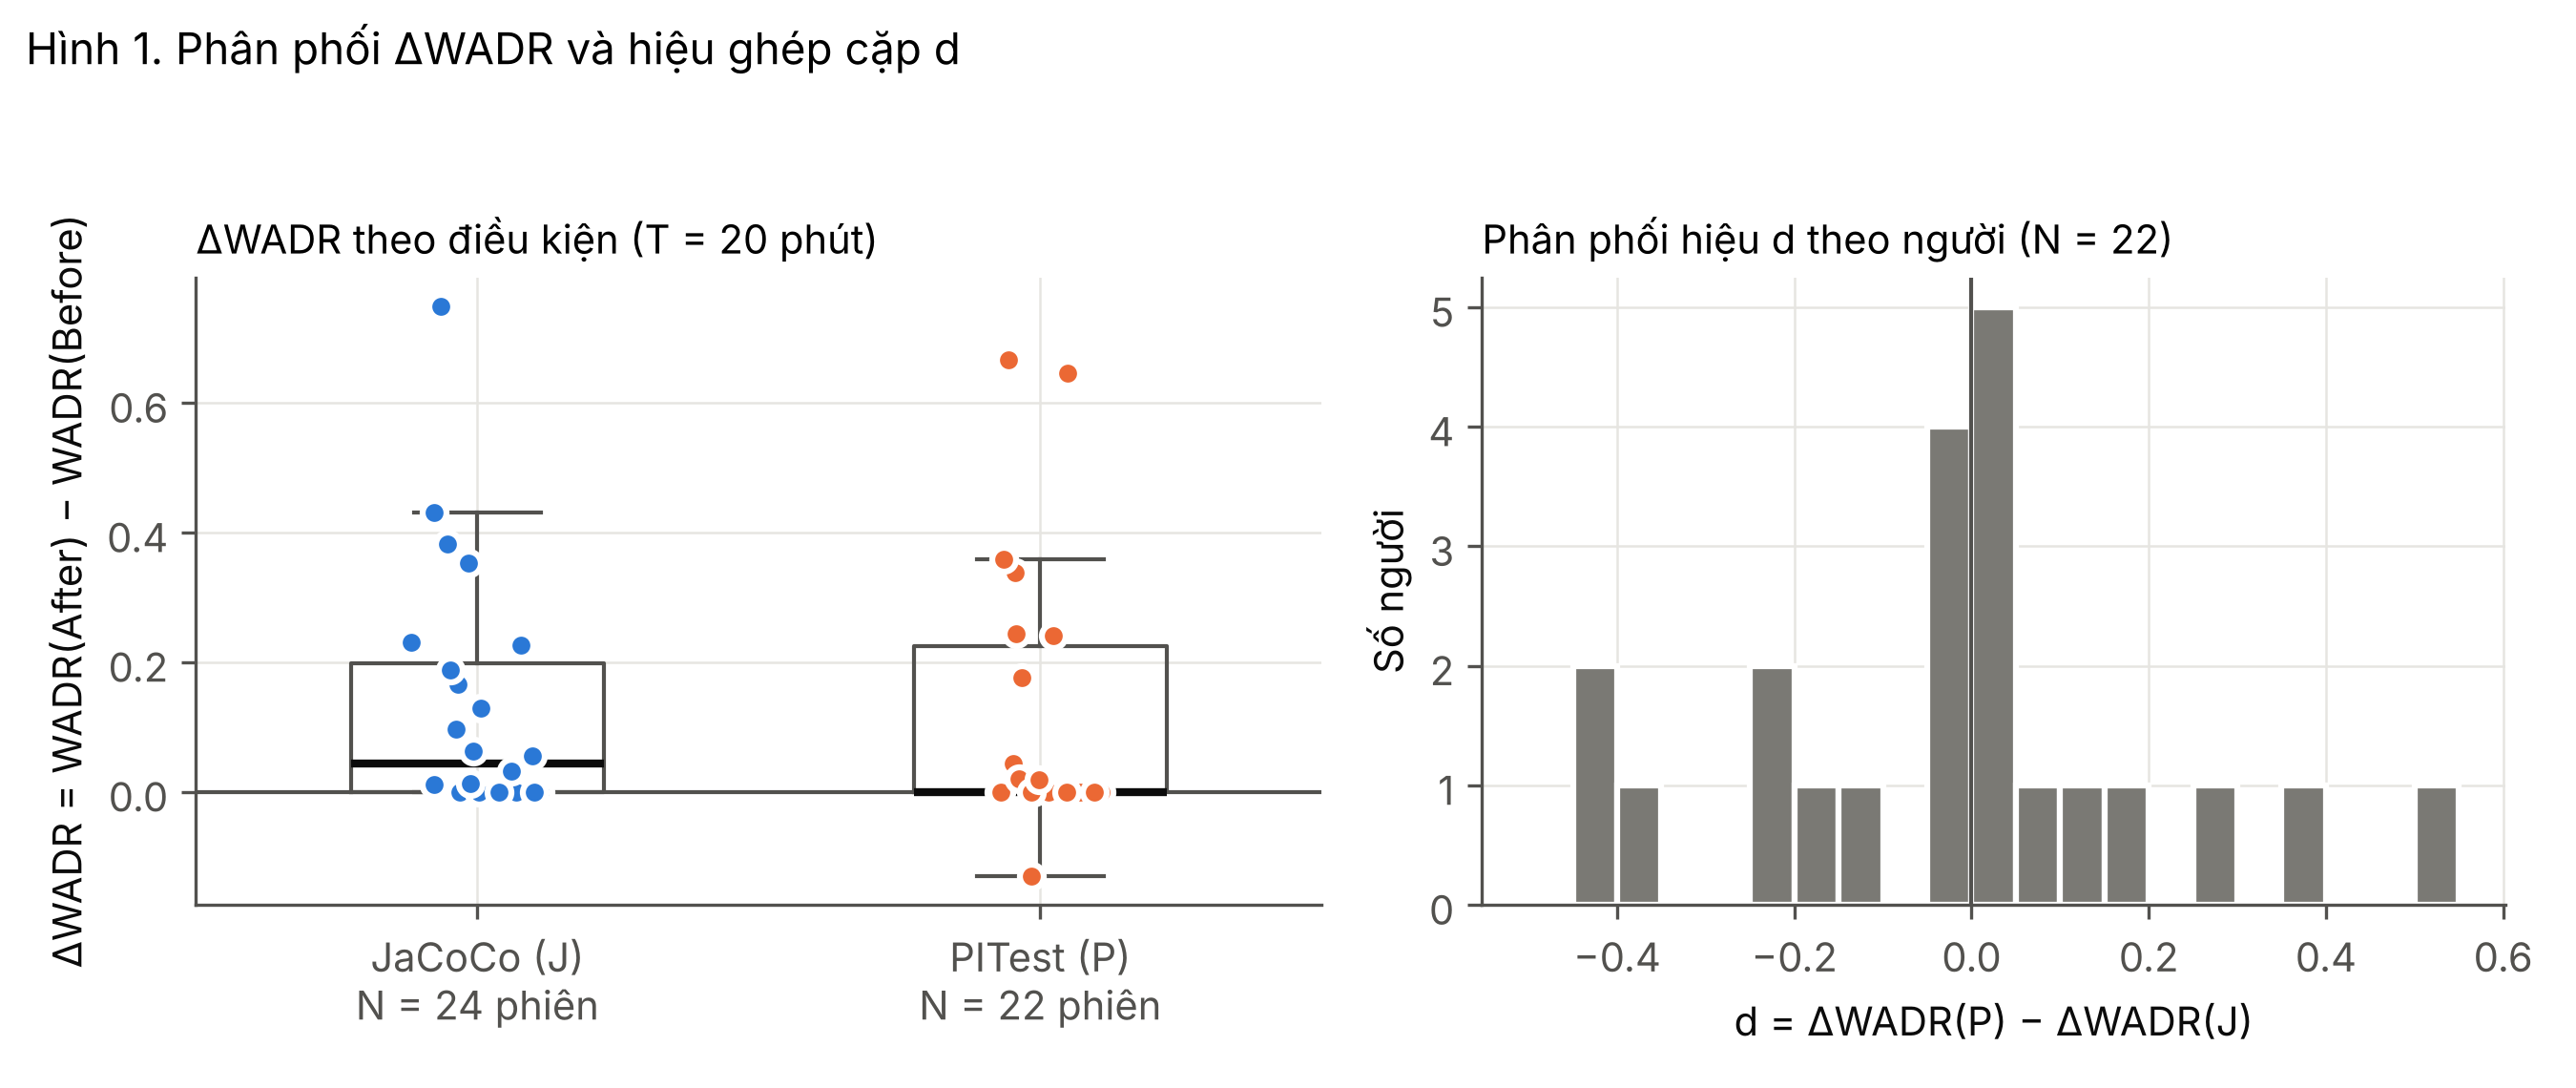
\includegraphics[width=\linewidth]{figures/fig1_distribution.png}
\caption{Left: $\Delta$WADR at $T = 20$ by condition (J: 24 sessions, P: 22 sessions). Right: paired difference $d$ per participant ($N = 22$).}
\label{fig:dist}
\end{figure}

\begin{figure}[t]
\centering
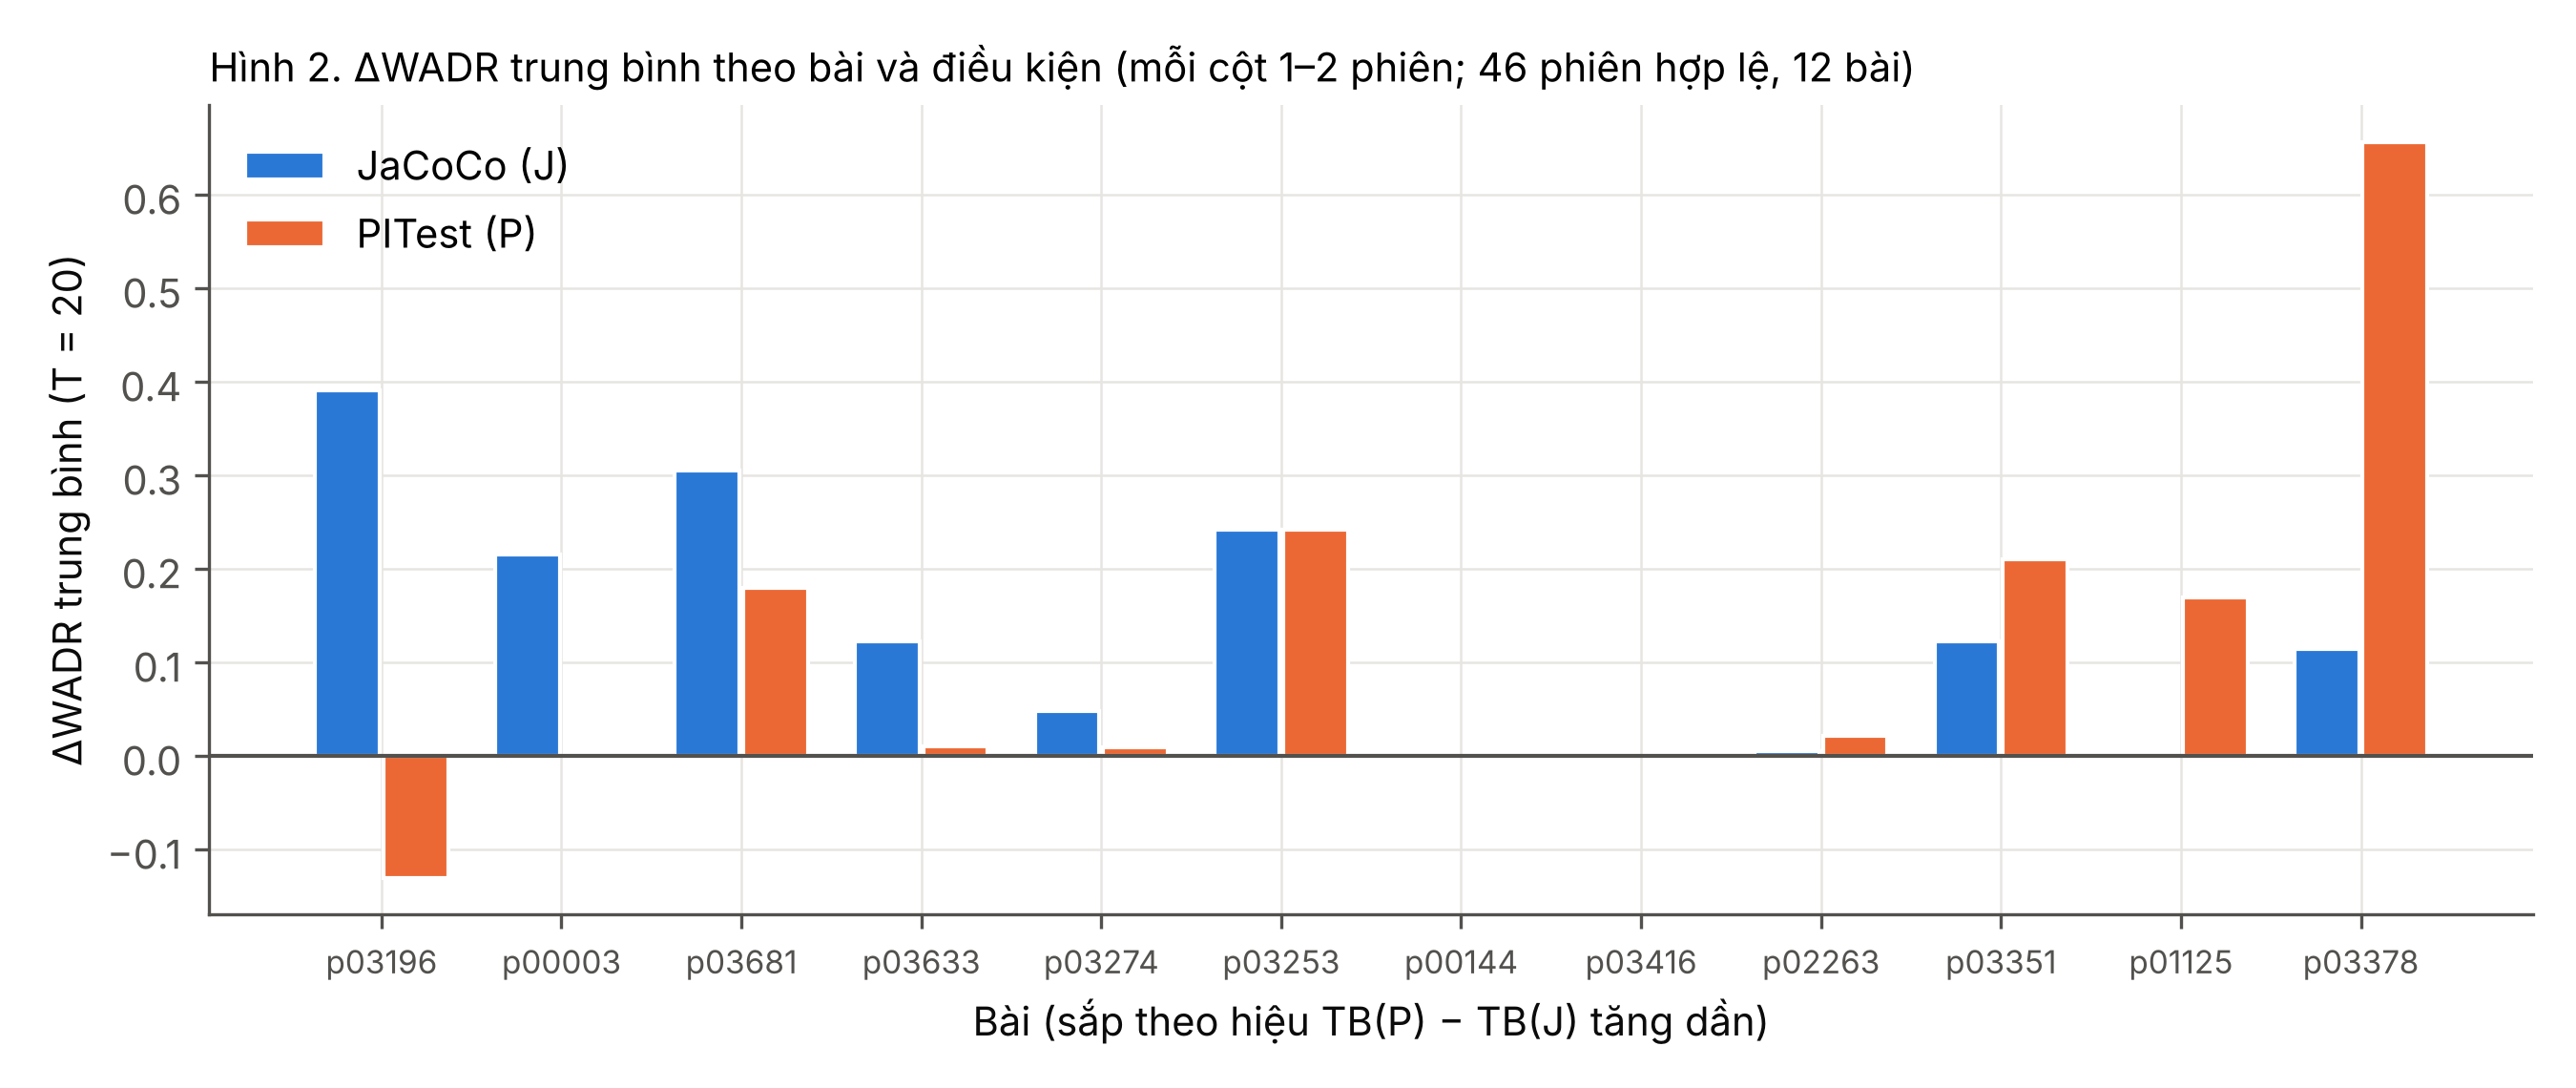
\includegraphics[width=\linewidth]{figures/fig2_comparison.png}
\caption{Mean $\Delta$WADR at $T = 20$ per problem and condition (one or two sessions per bar; 46 valid sessions, 12 problems).}
\label{fig:problem}
\end{figure}

\begin{table}[t]
\centering
\caption{Sessions excluded from the main paired analysis (\texttt{results/excluded.csv}).}
\label{tab:excluded}
\begin{tabular}{llll}
\hline
Session & Condition & Failure type & Reason \\
\hline
SV14-1 & P & method & After ($T = 20$) does not compile \\
SV14-2 & J & -- & partner session excluded \\
SV24-1 & P & method & After ($T = 20$) does not compile \\
SV24-2 & J & -- & partner session excluded \\
\hline
\end{tabular}
\end{table}


\section{Discussion}
\label{sec:discussion}

\subsection{Why the two feedback types did not differ}
A closer look at the 20 sessions with no gain ($\Delta$WADR = 0; 9 in J, 11 in P) suggests that the bottleneck was writing valid tests rather than choosing what to test.
In 17 of these 20 sessions, the After suite contained no valid input beyond those already in the Before suite; in the other 3, new valid inputs were added but caught no additional WA submission.
At T = 20, only 41\% of the tests in condition J and 43\% in condition P were valid.
Of the 249 invalid tests, 132 (53\%) failed on the correct program because the expected output was wrong, 81 (33\%) threw an exception on the correct program, typically because the input did not follow the required format, 34 (14\%) used inputs outside the problem constraints, and 2 timed out.
Both reports point to where a new test is needed, but neither tells the participant the correct expected output; if most new tests fail at this step, the type of report has little room to make a difference.

With its default configuration, PITest refuses to run when any test fails on the program under test, so in 58 of 96 runs participants in condition P saw an error message instead of a mutation report, while JaCoCo reported in every run.
Since a wrong expected value was the most common error, the same weakness that limited both conditions also removed the feedback in condition P.
In an exploratory comparison, P sessions that received at least one PITest report gained more (mean $\Delta$WADR 0.173, 11 sessions) than P sessions that received none (0.066, 11 sessions), but the paired estimate for those 11 participants still had a wide interval around zero ($\hat{\theta}$ = $-$0.020, 95\% CI [$-$0.212, 0.180]).
Tool run time is an unlikely explanation: a run took 6.9~s on average with JaCoCo and 7.2~s with PITest, which is small compared with the 20-minute budget.

\subsection{Comparison with prior work}
Alonge~\cite{alonge2025} reported a small advantage of mutation feedback over branch feedback, about 0.05 in the gain of conceptual mutants caught, with ten Python students in a between-group design.
Our interval includes differences of that size in both directions, so the two results do not conflict. A numeric comparison is not meaningful, though, because Alonge measured transfer on designed conceptual mutants after feedback was removed, whereas we measured held-out real WA submissions while feedback was in use.
The frequent absence of usable PITest reports is consistent with Mansur et al.~\cite{mansur2026}, who report that the unmodified PIT feedback did not meet students' needs, and with Shin and Kazerouni~\cite{shin2024}, who observed that mutation feedback can overload students and push them back to weaker strategies.
Studies in software engineering found that coverage and mutation score correlate only weakly with real fault detection once suite size is controlled~\cite{inozemtseva2014,papadakis2018}; in our data, the condition effect also stayed close to zero after controlling for the number of independent inputs ($-$0.028, Section~\ref{sec:results}).

\subsection{Implications}
These results suggest that, for short exercises on small programs, instructors should not expect a large difference between the two reports in how many real wrong submissions the added tests catch.
Instructors who use PITest should make sure students can act on its output, for example by showing which tests fail on the correct program before mutation analysis runs, since otherwise many students receive no mutation report at all.
Teaching students to check expected outputs against the problem statement may matter more than the choice of report.
For researchers, the share of runs in which each tool actually produced feedback should be reported, because a null result may come from missing feedback rather than from feedback that did not help.

\subsection{Unexpected result}
We did not anticipate that PITest would stop on failing tests in most runs; the protocol assumed that every session would receive a report with content (Section~3).
This deviation is reported in Section~\ref{sec:results} and in \texttt{notes.md}.

\subsection{Lessons from running the experiment}
During the runs, we found that the planned sample of 48 could not be reached within the schedule, so the study is reported as exploratory with 24 participants, as the protocol allows.
The grader, locked manifests and pre-registered analysis rules made it possible to rerun every analysis from the stored session files, and all checks of the session data against the schedule and the locked manifests passed.

\section{Threats to Validity}
\label{sec:threats}

\textbf{Internal validity.}
Participants may carry skills from the first session into the second, or tire during it. We counterbalanced tool order in the crossover schedule and used a different problem in each session. The crossover regression estimated a period effect of 0.004 (p = 0.934), but with 22 participants this test has little power, so a carry-over effect cannot be ruled out.
A second threat is that PITest produced no report in 58 of 96 runs because a test failed on the program. The comparison is therefore between JaCoCo reports and PITest as users actually experience it with its default configuration, not between two complete reports. We report the share of runs with a report per condition, plus an exploratory analysis restricted to participants who received at least one PITest report.

\textbf{External validity.}
All tasks were small Java programs from IBM CodeNet~\cite{puri2021}, selected so that both tools report items that reference inputs can cover or kill. Results may differ for larger programs, other languages or other problem types.

\textbf{Construct validity.}
WADR counts detected WA submissions, not distinct faults, so several submissions may share one fault.
The oracle is the output agreed by at least 90\% of Accepted solutions, together with four independent Accepted solutions per problem. It can still be wrong on rare valid inputs. Three tests disagreed with the reference solutions, and WADR was the same whether they were kept or removed. We did not review these three tests manually, because the result does not depend on them.
A validator removed tests outside the problem constraints. Inputs that the validator accepts but the problem does not intend may remain.

\textbf{Conclusion validity.}
With N = 22 participants in the main analysis, the simulation in the protocol gives a minimum detectable effect between 0.07 and 0.23, depending on the assumed variability. A true difference of $\delta$ = 0.10 could therefore easily be missed. We report the estimate with its 95\% confidence interval ([$-$0.118, 0.074]) and do not claim that the two feedback types are equivalent, since no equivalence test was pre-registered.
Problems are shared between participants, so the paired differences are not fully independent. The mixed model with problem as a fixed effect gave the same conclusion.

\section{Conclusion}
\label{sec:conclusion}

We compared uncovered-branch feedback from JaCoCo with surviving-mutant feedback from PITest in a crossover experiment. Twenty-four participants added JUnit tests to two CodeNet programs under the same 20-minute budget, and we measured the gain in detection of held-out real Wrong Answer submissions.
We found no difference between the two feedback types ($\hat{\theta}$ = $-$0.012, 95\% CI [$-$0.118, 0.074], p = 0.483, N = 22), and all pre-specified sensitivity analyses agreed.
Two things limit this result. Most added tests were invalid, mainly because of wrong expected outputs. And with its default configuration, PITest produced no report in 58 of 96 runs because of failing tests.

Future work should (1) repeat the experiment with students in a software testing course, using the 48 participants planned in the protocol, to reach a minimum detectable effect near $\delta$ = 0.10; (2) run PITest only on tests that pass on the program under test, so that every P session receives a mutation report, and compare this configuration with the default; and (3) give both groups a way to check expected outputs, to test whether the report type matters once tests are valid.


\section*{Conflict of Interest}
The authors declare no conflict of interest.

\section*{Data Availability}
The frozen problem list, WA manifests, session data, grading and analysis scripts, and the analysis notebook are available in the project repository (RT-SWT301-004-nhom3).

\bibliographystyle{plain}
\bibliography{references}
\end{document}
